\documentclass[../Main/Knit.tex]{subfiles}
\newpage
\subsection{Bioinformatics Pipeline}
Unlike the Iso-Seq bioinformatics pipeline which was largely established by PacBio, the pipeline for processing ONT reads was less defined and streamlined with constant emergence of new tools from research community. Much of the analysis, such as the usage of \textit{Porechop} to remove primer sequences and of \textit{TAMA} for transcript collapse, was taken from the Wellcome Trust Advanced Course: RNA Transcriptomics (2018), provided by J.Ragoussis (referred as WTAC), and refined using ERCC as benchmark. 

\begingroup
\parindent=0em
\etocsettocstyle{\rule{\linewidth}{\tocrulewidth}\vskip0.5\baselineskip}{\rule{\linewidth}{\tocrulewidth}}
\etocsetnexttocdepth{5}
\localtableofcontents 
\endgroup

\subsubsection{Base-calling}
The first analysis is to convert or "base-call" the electrical signals to the corresponding bases using Albacore, or a more recently developed package, Guppy, that requires information on the: 
\begin{enumerate}
	\item Chemistry of the run such as whether 1D or 1D\textsuperscript{2}
	\item Flow cell version used, to define the protein nanopore and subsequent 6-mer, which has different residual current	
	\item Sequencing kit used as this specifies the translocation speed, which informs the event segmentation algorithm how to recognise the corresponding bases from the electrical signal
	\item use of barcoding to run multiple samples in one flow cells for downstream demultiplexing
	\item type of output file, such as FASTQ or fast5
\end{enumerate}
In contrast to PacBio's SMRT with the ability to generate consensus long reads, the raw accuracy of nanopore 1D cDNA sequencing is relatively low between 85–87\%; however, significant improvements are made on reducing error rate by rapid development of both the technology and library preparation methods (Volden et al. 2018). Such high error rates, from frequent base deletions and insertions particularly near splice sites, can result in spurious alignments and in correct clustering of reads. 


\subsubsection{Quality Control of Run and Filtering of Base-called Reads}
The quality characterisations of a single Nanopore sequencing run was assessed using \textit{PycoQC}\cite{Leger2019} and the official Nanopore QC tutorial\cite{ONT2019NanoporeQC}, by evaluating the performance of the run, the number of reads generated over time, and the length and quality score distribution of basecalled reads. Reads with read quality score < 7 were removed using \textit{Nanofilt}\cite{DeCoster2018} with default parameters.


\subsubsection{Removing of Nanopore and cDNA sequencing adapters}
Similarly to the Iso-Seq bioinformatics pipeline, cDNA sequencing primer sequences and nanopore ligation adaptors were removed to prevent spurious alignment, using \textit{Porechop}\cite{Wick2017} (v0.2.4, parameters: --end\_size 100, --adapter\_threshold 90, --end\_threshold 75, --min\_trim\_size 15, --discard\_middle, --extra\_end\_trim 1). Under those parameters, a window of 100 nucleotides from each end of the reads were searched for a set of adaptors, which must have a minimum 90\% identity to be considered present for trimming and a minimum 75\% at the end of the reads; alignments smaller than 15bp or found within the middle of the reads (considered chimeric) were removed. By manually defining a unique set of adaptors that includes the cDNA primers (from Clontech SMARTer PCR cDNA synthesis kit), the ONT adaptors and corresponding polyA/T tail, it was possible to differentiate the strand orientation (Figure \ref{fig:ONT_cdnatemplate}). Trimmed reads with adaptors present at both ends were retained, and reads corresponding to the minus strand were reverse complemented. Using \textit{Cutadapt}\cite{Martin2011} (v2.9, -a "A{40}"), the polyA sequence was then trimmed 40 nucleotides from the 3'end.

Of note, \textit{Porechop} has been officially unsupported since 2018 and has been largely replaced by ONT's officially recommended tool, \textit{Pychopper}\cite{OxfordNanoporePychopper}; however, \textit{Pychopper} was not able to differentiate the strands for classification given that the 5'ends of both plus and negative strands have the same sequence (due to the nature of the cDNA synthesis kit). 

\begin{figure}[htp]
	\begin{center}
		\includegraphics[page=7,trim={2cm 17cm 0cm 1cm},clip, scale = 0.55]{Pictures/Pipeline.pdf}
	\end{center}
	\captionsetup{width=0.95\textwidth}
	\caption[Structure of ONT library cDNA template]%
	{\textbf{Structure of ONT library cDNA template}: Shown is the \textbf{a)} final structure of cDNA molecules for ONT sequencing, after cDNA synthesis and adaptor ligation, and the corresponding differentiating start and end sequence for the plus and minus strands \textbf{b)} without and \textbf{c)} with barcodes. The original cDNA molecules are outlined in purple and green, and the ONT boxes indicate the position of the ONT adaptors. In cases where multiplexing is performed, the barcode location is indicated in red (see \cref{tab:barcode_primers} and \cref{tab:ont_barcode} for barcode sequences). Of note, only the plus strand end sequence and the minus strand start sequence contain the barcode and are used for sample demultiplexing, whereas the plus strand start and minus strand end sequence are identical across all barcoded samples. The brown and orange circle refer to the motor protein and cholesterol moiety respectively. The start and end of the strand is defined by the 5' and 3' end respectively. }
	\label{fig:ONT_cdnatemplate}
\end{figure}

\begin{landscape}
	\begin{table}[]
		\centering
		\begin{tabular}{@{}ccccc@{}}
			\toprule
			\multirow{2}{*}{Barcoded  Samples} & \multicolumn{2}{c}{Plus strand} & \multicolumn{2}{c}{Minus strand} \\ \cmidrule(l){2-5} 
			& Start sequence & End sequence & Start sequence & End sequence \\ \midrule
			BC1 & \multirow{10}{*}{\begin{tabular}[c]{@{}c@{}}TTGCTAAG\\ CAGTGGTA\\ TCAACGCA\\ GAGTACAT\\ GGG\end{tabular}} & AAAAAACGCACTCTGATATGTGGCA & CACATATCAGAGTGCGTTTTTT & \multirow{10}{*}{\begin{tabular}[c]{@{}c@{}}CCCATGTAC\\ TCTGCGTTG\\ ATACCACT\\ GCTTAGCAAT\\ ACGTAACT\end{tabular}} \\
			BC2 &  & AAAAAAACTCACAGTCTGTGTGTGCA & ACACACAGACTGTGAGTTTTTTT &  \\
			BC3 &  & AAAAAAACTCTCACGAGATGTGTGCA & ACACATCTCGTGAGAGTTTTTTT &  \\
			BC4 &  & AAAAAAACGCGCGTGTGTGCGTGGCA & CACGCACACACGCGCGTTTTTTT &  \\
			BC5 &  & AAAAAAAACGCGAGAGTCGAGTGGCA & CACTCGACTCTCGCGTTTTTTTT &  \\
			BC6 &  & AAAAAAAACAGCTGATATATATGGCA & CATATATATCAGCTGTTTTTTTT &  \\
			BC7 &  & AAAAAAACACATAGAGATACAGAGCA & TCTGTATCTCTATGTGTTTTTTT &  \\
			BC8 &  & AAAAAAACGCAGCGCTCGACTGTGCA & ACAGTCGAGCGCTGCGTTTTTTT &  \\
			BC9 &  & AAAAAAATCTGTCTCGCGTGTGTGCA & ACACACGCGAGACAGATTTTTTT &  \\
			BC10 &  & AAAAAAACTCTGAGATAGCGCGTGCA & ACGCGCTATCTCAGAGTTTTTTT & 
		\end{tabular}
	\captionsetup{width=0.9\linewidth}
	\caption[ONT adapter sequences for plus and minus strand of barcoded samples]%
	{\textbf{ONT adapter sequences for plus and minus strand of barcoded samples}. Tabulated are the sequences used in \textit{Porechop} for sample demultiplexing and identifying the plus and minus strands. As depicted in \cref{:ONT_cdnatemplate}, only the plus strand end sequences and the minus strand start sequences contain the sample-specific barcode sequence (reverse complementary of one another). BC - Barcode}
	\label{tab:ont_barcode}
	\end{table}
\end{landscape}

\subsubsection{Genome Alignment and Transcript Collapse}
Trimmed reads were then aligned to the reference genome using Minimap2 \cite{Li2018} (v2.17-r941, parameters: -ax splice). In the Iso-Seq bioinformatics pipeline, mapped transcripts were then processed using \textit{Cupcake} for the removal of transcripts with low alignment identity and length, further collapse of high-quality transcripts to unique isoforms, and to obtain count information using output from \textit{IsoSeq3 Cluster}.

As a similar comparison, mapped transcripts from ONT were processed using \textit{TAMA} for removal of lowly-aligned transcripts and for further collapse to unique isoforms (script: tama\_collapse.py, parameters: -e common\_ends, -c 95, -i 80, -x capped -a 50, -z 50, -m 20, -d merge\_dup) and to subsequently obtain count information (script: tama\_read\_support\_levels.py). Under those parameters recommended by WTAC, transcripts were filtered for minimum alignment identity > 80\% and alignment length >95\% (same threshold as that applied in Iso-Seq pipeline using \textit{Cupcake}) and collapsed by common exon start and end sites. 50 nucleotides at both 5'end and 3' end of the transcript, and 20 nucleotides at the exon/splice junction and tolerated for grouping transcripts to be collapsed. Of note, this is much more relaxed than the default \textit{TAMA} parameters (-a 10 -m 10 -z 10), given that the 5'cap method was not used and the error rate of ONT reads were high. 

Despite the growing emergence of various new tools developed for processing ONT reads - such as ONT's officially recommended pipeline with Pinfish and Stringtie, FLAIR, UNAGI - I chose to use \textit{TAMA} due to greater flexibility and transparency with parameter usage, generation of multiple output files for quality control, and ability to subsequently obtain count information (script: tama\_read\_support\_levels.py)


\uline{\textbf{FLAIR}}: Full-Length Alternative Isoform analysis of RNA  (FLAIR\nomenclature{FLAIR}{Full-Length Alternative Isoform analysis of RNA}) 
Three steps are involved: Correct splice sites with short reads if incorrect splice site is within 10base pairs away from correct splice site, collapse reads to generate consensus sequences. This involves first grouping reads with identical splice junctions - "first pass nanopore isoform transcriptome"; the representative isoform within each group is determined by the most supported transcription and end site. All the reads, including reads that were aligned but not able to be fully corrected, are re-aligned to the "first-pass isoform" with the best alignment. First-pass isoforms that have fewer than three supporting reads are filtered out; three supporting reads selected as threshold as this gave the highest base sensitivity without compromising on precision.  

\subsubsection{Isoform Quantification} 
In contrast to Iso-Seq, isoform quantification from ONT is relatively simpler in that each nanopore read corresponds to a single transcript (Tang et al. 2020). However, ambiguity still remains with assignment of truncated reads 

\subsubsection{Limitations of Oxford Nanopore} 
Refer to \cite{Workman2019a} for information on strand break etc